\section{Other approaches}

\subsection{Learning-based frameworks for link prediction}

Earlier described approaches (e.g., similarity and probabilistic
methods) deal with the computing a score of each non-observed link
either by a similarity or a probabilistic function. However, \textbf{the
    link prediction problem can also be modeled as a learning-based model}
to exploit graph topological features and attribute information. The
problem is cast as a \textbf{supervised classification model} where a
\textbf{point} (i.e., training data) \textbf{corresponds to a
    vertex-pair in the network}, and the \textbf{label} of the point
\textbf{represents the presence or absence of an edge (link) between the
    pair}.\\ In other words, \emph{consider a vertex-pair} \(\mathit{(x, y)}\)
\emph{in the graph} \(\mathit{G(V, E)}\) \emph{and the label of the
    corresponding data point in the classification model is}
\(\mathit{l_{(x,y)}}\) . Then,

\[l_{(x, y)}=
    \begin{cases}
        +1 \ \text{ if } (x, y) \in E \\
        -1 \ \text{ if } (x, y) \notin E
    \end{cases}
\]

\textbf{This is typically a binary classification task} where several
classifiers (e.g.,
\texttt{decision\ tree,\ naive\ Bayes,\ support\ vector\ machine}, etc.)
can be employed to predict the label of unknown data points
(corresponding to missing links in the network). One of the major
challenges of this model (i.e., machine learning) is the
\textbf{selection of appropriate feature set}. Majority of the existing
research works extract feature sets from the network topology (i.e.,
topological information of the network). These \textbf{features are
    generic} and domain-independent that are \textbf{applicable to any
    network}. Such features are typical,
\texttt{neighborhood,\ and\ path-based\ features}.\\ Some other works
concentrate on extracting node and edge features that play a crucial
role to improve the performance of link prediction. The cost of
extraction of such features is cheap and easy, while the main
disadvantage is the domain-specific nature of them.

\subsection{Information theory-based link prediction}

Several complex networks have utilized the concept of
\textbf{information theory to compute their complexity on different
    scales}. They defined several correlation measures and modeled some
networks (e.g., \texttt{star,\ tree,\ lattice,\ ER\ graph}, etc.).
\textbf{Bauer et al.} used the \texttt{maximum\ entropy\ principle} to
assign a statistical weight to any graph and introduced random graph
construction with arbitrary degree distribution.\\

\textbf{Tan et al.} posed the link prediction problem in the
\texttt{framework\ of\ information\ theory}. They mainly focus on local
assortativity to capture local structural properties of the network and
showed that \texttt{mutual\ information\ (MI)} method performs well on
both low and highly correlated networks. Motivated by, \textbf{Zhu, B.
    and Xia} added more local features (i.e., links information of neighbors
of the seed nodes as well as their common neighbors) in their framework
and called it as \texttt{neighbor\ set\ information\ (NSI)\ index}.
Thus, they showed that the different features could be combined in an
information-theoretic model to improve the link prediction accuracy.\\

\textbf{Xu et al.} considered path entropy as a similarity metric for
the link prediction problem. The authors assumed that there is no
correlation among the degrees of the nodes in the network. Consider the
following notations based on their paper: \(L^0_{xy}\) shows no link
exists between two vertices \(x\) and \(y\), and the corresponding
existence is represented by \(L^1_{xy}\). Probability of existence of a
link between the above two vertices is given as

\[
    P(L^1_{xy}) = 1 - P(L^0_{xy}) = 1 - \frac{C^{k_y}_{M-k_x}}{C^{k_y}_M}
\]

where \(C_M^{k_Y}\) represents the number of candidate link sets for the
vertex \(y\) with all links incident with \(y\) and \(C^{k_y}_{M-k_x}\)
denotes the number of candidate link sets for the vertex \(y\) with all
links incident with \(y\) but none of them is incident with \(x\).
Outcome results on several networks demonstrate that the similarity
index based on path entropy performs better than other indices in terms
of prediction accuracy and precision. \textbf{Xu et al.} extend the
previous work to the weighted network by considering the weight of the
paths. Recently, some more efforts have been applied in this direction
based on different features of the networks like influential nodes,
combining node attributes with
\texttt{structural\ similarity,\ local\ likelihood,\ and\ maximal\ entropy\ random\ walk}.

\subsection{Clustering-based Link Prediction}

\textbf{Huang} presented a paper on
\texttt{graph\ topology-based\ link\ prediction} where a
\texttt{generalized\ clustering\ coefficient} is used as a
\textbf{predictive parameter}. The author introduces a \textbf{cycle
    formation model} that shows the relationship between link occurrence
probability and its ability to form different length cycles. This model
suggests that the occurrence probability of a particular link depends on
the number of different lengths cycles formed by adding this link. The
model is based on the assumption of the stationary property of the
degree of clustering of the network. This model captures longer cycles
by extending the higher-order clustering coefficients and defines the
generalized clustering coefficient \(C(k)\) as

\[C(k) = \frac{\textit{number of j-length cycles}}{\textit{number of k-length paths}}\]

where \(k\) is the \textbf{degree} of the cycle formation model.

The author treats the link occurrence probability as governed by \(t\)
link generation mechanisms \(g(1), g(2),...,g(k)\) of cycle formation
model, each described by a single parameter \(c_1, c_2,...,c_k\) . The
above mentioned link generation mechanism can be understood with the
help of the Figure below.

\begin{figure}[H]
    \centering
    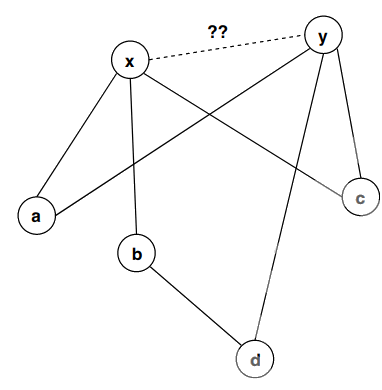
\includegraphics[width=7cm, keepaspectratio]{capitoli/methods/imgs/img6.png}
    \caption{An example illustrating the cycle formation link probability model.}
\end{figure}

Consider a cycle formation model ( \(CF (k)\) ) of degree \((k = 3)\).
The Seed link \((x, y)\), here, can be generated by the following three
mechanisms: - \texttt{random\ link\ occurrence\ g(1)} -
\texttt{length-2\ cycle\ generation\ g(2)}
i.e.~\((x −a −y and x −c −y)\) -
\texttt{length-4\ cycle\ generation\ g(3)} i.e.~\((x −b −d −y)\).

The main issue is to combine several generation mechanisms to compute
total link occurrence probability. The author posits a method to combine
both path and cycle (of different lengths) generation mechanism in the
framework. The expected general clustering coefficient of degree \(k\)
for this model can be estimated as
\[E[C(k)] = f(c_1, c_2, ..., c_k) = \sum_{i} |G_i|p(G_i)p((e_{l, k+1} \in E|G_i)) \]
where \(|G_i|\) is the number of subgraph possible corresponding to the
graph pattern \(G_i\), \(p(G_i)\) is the probability of occurrence of
one of such graphs \(G_i\), and \(p(e_{l,k+l})\) is the probability of
edge \(e_{l,l+1}\) to occur given the pattern \(G_i\). Finally, given
the coefficients, the probability of existence of link is
\[p_{x,y}(c_1, ..., c_k) = \frac{c_1 \prod_{i=2}^{k} c_i^{|path^i_{x,y}|}}{c_1 \prod_{i=2}^{k} c_i^{|path^i_{x,y}|} + (1-c_1)\prod_{i=2}^{k} (1-c_i)^{|path^i_{x,y}|}}\]

\textbf{Liu et al.} proposed degree related clustering coefficient to
quantify the clustering ability of nodes. They applied the same to paths
of shorter lengths and introduced a new index
\texttt{Degree\ related\ Clustering\ ability\ Path\ (DCP)}. They
performed the \texttt{degree\ of\ robustness\ (DR)} test for their index
and showed that missing links have a small effect on the index. Recently
\textbf{Wu et al.} extracted triangle structure information in the form
of node clustering coefficient of common neighbors. Their experiments on
several real datasets show comparable results to the \texttt{CAR} index.
The same concept of the clustering coefficient also introduced in the
work presented by \textbf{Wu et al.}. Authors introduce both node and
link clustering information in their work. Their experiments on
different network datasets showed better performance results against
existing methods, especially on middle and large network datasets.
\textbf{Kumar et al.} explored the concept of node clustering
coefficient to the next level (level-2) that captures more clustering
information of a network. The comprehensive results on several
real-world datasets show better performance compared to local methods
and comparable to the node embedding method \texttt{Node2vec}.
Meanwhile, \textbf{Benson et al.} studied simplicial closure events to
capture higher-order structures in several temporal networks. The
simplicial closure events are the process of closure of timestamped
simplices (simplicial complexes 2 are set of nodes with different sizes)
available in a dataset. These structures are common in several real-time
complex systems, for example, communication in a group, collaboration of
authors for a paper, etc. To assess these higher-order structures, the
authors study the simplicial closure events on triples of nodes (for
simplicity) and suggest that the open triangles or triples of nodes with
strong ties are more likely to close in the future.

\subsection{Structural Perturbation Method}

\textbf{\emph{Lu et al.}} introduced a new framework of computing
predictability of links in the networks. They coined a
\textbf{structural consistency index} to quantify the link
predictability. This index is based on the assumption that ``\emph{links
    in a network are highly predictable if no significant changes occur in
    the structural feature after the addition or deletion of a small
    fraction of the link}''. Based on this index, they proposed a new
similarity index, namely
\texttt{structural\ perturbation\ method\ (SPM)}. The experimental
results show the outstanding performance compared to the
state-of-the-art in their paper.